\documentclass{article}
\usepackage[utf8]{inputenc}
\usepackage{amssymb}
\usepackage{amsfonts}
\usepackage{amsmath}
\usepackage[utf8]{inputenc}
\usepackage[norsk]{babel}
\usepackage{lmodern}
\usepackage{float}
\usepackage{graphicx}
\DeclareGraphicsExtensions{.pdf,.png,.jpg}
\usepackage{latexsym}
\usepackage{hyperref}
\usepackage[euler]{textgreek}
\usepackage{stackengine}
\usepackage[version-1-compatibility]{siunitx}
\usepackage{pdfpages}
\usepackage{fixltx2e}
\hypersetup{pdfborder={0 0 0}}
\usepackage{pgfplots}
\pgfplotsset{compat=newest}
\pgfplotsset{plot coordinates/math parser=false}
\newlength\figureheight
\newlength\figurewidth
\usepackage[section]{placeins}%Sørger for at plots og andre floats holder seg til sin section.
\setlength\parindent{0pt}%Setter indent til 0



\title{Exercise 3 - TTK4130 Modeling and Simulation}
\author{Camilla Sterud}
\date{}

\begin{document}

\maketitle

\newpage

\section{Problem 1}



\subsection{a}


\begin{figure}[!ht]
    \centering
    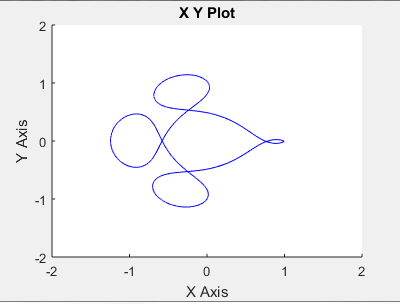
\includegraphics[width = 0.5\textwidth]{step_0025}
    \caption{1 round with ode5 solver. h = 0.0025. It's ok.}
\end{figure}



\end{document}